% ==============================================================================
% 第五章: 作弊条 - 所有无脑公式汇总
% ==============================================================================
\section{作弊条 (考前看这页)}

\subsection{2的幂次表}

\begin{center}
\begin{tabular}{|c|c|c|c|c|c|c|c|}
\hline
$2^4$ & $2^5$ & $2^6$ & $2^7$ & $2^8$ & $2^9$ & $2^{10}$ & $2^{16}$ \\
\hline
16 & 32 & 64 & 128 & 256 & 512 & 1024 & 65536 \\
\hline
\end{tabular}
\end{center}

\subsection{数值范围}

\begin{center}
\begin{tabular}{|c|c|c|}
\hline
位数 & Unsigned & Signed \\
\hline
8 & 0$\sim$255 & $-128\sim+127$ \\
10 & 0$\sim$1023 & $-512\sim+511$ \\
16 & 0$\sim$65535 & $-32768\sim+32767$ \\
\hline
\end{tabular}
\end{center}

\subsection{数值计算速查}

\begin{center}
\fbox{\parbox{0.9\linewidth}{
\textbf{Unsigned溢出:} 结果 \% $2^N$

\textbf{Signed溢出:} 结果 $> 2^{N-1}-1$?减$2^N$

\textbf{负数补码:} $2^N - |X|$

\textbf{补码转值:} MSB=1? 值$-2^N$
}}
\end{center}

\subsection{K-Map位置}

\begin{center}
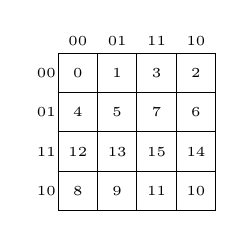
\begin{tikzpicture}[scale=0.5]
\draw (0,0) grid (4,4);
\node at (0.5, 4.3) {\tiny 00};
\node at (1.5, 4.3) {\tiny 01};
\node at (2.5, 4.3) {\tiny 11};
\node at (3.5, 4.3) {\tiny 10};
\node at (-0.3, 3.5) {\tiny 00};
\node at (-0.3, 2.5) {\tiny 01};
\node at (-0.3, 1.5) {\tiny 11};
\node at (-0.3, 0.5) {\tiny 10};
\node at (0.5,3.5) {\tiny 0};
\node at (1.5,3.5) {\tiny 1};
\node at (2.5,3.5) {\tiny 3};
\node at (3.5,3.5) {\tiny 2};
\node at (0.5,2.5) {\tiny 4};
\node at (1.5,2.5) {\tiny 5};
\node at (2.5,2.5) {\tiny 7};
\node at (3.5,2.5) {\tiny 6};
\node at (0.5,1.5) {\tiny 12};
\node at (1.5,1.5) {\tiny 13};
\node at (2.5,1.5) {\tiny 15};
\node at (3.5,1.5) {\tiny 14};
\node at (0.5,0.5) {\tiny 8};
\node at (1.5,0.5) {\tiny 9};
\node at (2.5,0.5) {\tiny 11};
\node at (3.5,0.5) {\tiny 10};
\end{tikzpicture}
\end{center}

\textbf{顺序:}00-01-11-10

\textbf{圈大小:}1,2,4,8,16

\textbf{四角可以圈!}

\subsection{RS锁存器}

\begin{center}
\begin{tabular}{|cc|c|}
\hline
S & R & Q \\
\hline
0 & 0 & 保持 \\
0 & 1 & 0 \\
1 & 0 & 1 \\
1 & 1 & 禁止 \\
\hline
\end{tabular}
\end{center}

\textbf{口诀:}S高Q高,R高Q低

\subsection{香农展开}

\begin{center}
\fbox{$F = \bar{A}F_0 + AF_1$}
\end{center}

$F_0$:A换0,$\bar{A}$换1

$F_1$:A换1,$\bar{A}$换0

\subsection{流水线连连看}

\begin{center}
\begin{tabular}{|l|l|}
\hline
Data Hazard & Forwarding \\
Load-Use & Stall \\
Branch & Flush \\
\hline
\end{tabular}
\end{center}

\textbf{CPI} = 1 + Stall率

\textbf{5级:}IF-ID-EX-MEM-WB

\subsection{布尔代数}

\begin{center}
\begin{tabular}{|l|l|}
\hline
$\overline{A+B}=\bar{A}\bar{B}$ & 德摩根 \\
$\overline{AB}=\bar{A}+\bar{B}$ & 德摩根 \\
$A+AB=A$ & 吸收律 \\
$A+\bar{A}B=A+B$ & 互补 \\
$A\oplus B=A\bar{B}+\bar{A}B$ & 异或 \\
\hline
\end{tabular}
\end{center}

\vfill
\begin{center}
\textbf{\large Good Luck!}

\small 2026-01-13 10:00 | KN-A-310

\textit{兄弟,稳住,你能行的!}
\end{center}
